\subsection{Experimentaci\'on ``Aleatoria''}

\subsubsection{An\'alisis de complejidad}
\begin{figure}[H] 
    \centering
    \begin{minipage}{0.45\textwidth}
        \centering
        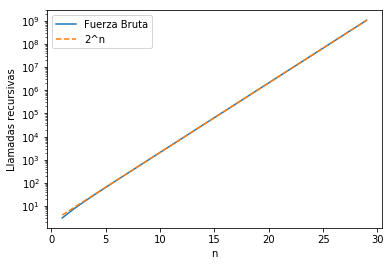
\includegraphics[width=1\textwidth]{img/complejidad/llamadasFB.png} % first figure itself
        \caption{Comparaci\'on de Fuerza Bruta con $2^n$ (Complejidad te\'orica)}
        \label{fig:llamadasFB}
    \end{minipage}\hfill
    \begin{minipage}{0.45\textwidth}
        \centering
        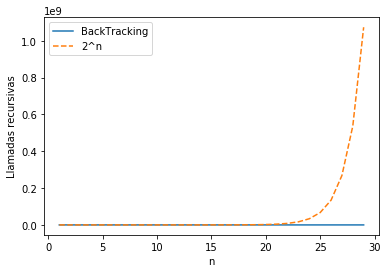
\includegraphics[width=1\textwidth]{img/complejidad/llamadasBack.png} % first figure itself
        \caption{Comparaci\'on de BackTracking con $2^n$ (Complejidad te\'orica)}
        \label{fig:llamadasBack}
    \end{minipage}\hfill
\end{figure}
\begin{figure}[H] 
    \centering
    \begin{minipage}{0.45\textwidth}
        \centering
        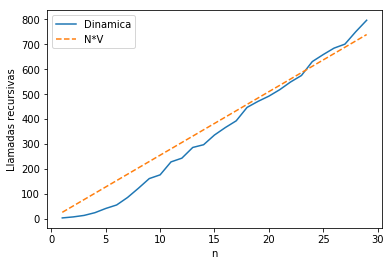
\includegraphics[width=1\textwidth]{img/complejidad/llamadasDin.png} % first figure itself
        \caption{Comparaci\'on de Programaci\'on Din\'amica con $n*V$ (Complejidad te\'orica)}
        \label{fig:llamadasDin}
    \end{minipage}\hfill
\end{figure}

\par Analizando los gr\'aficos podemos ver que en la Figura \ref{fig:llamadasFB} la complejidad del algor\'itmo de Fuerza
Bruta se solapa perfectamente con el de la complejidad te\'orica esperada.
\par Por otro lado, viendo la Figura \ref{fig:llamadasBack} se puede apreciar que la complejidad est\'a muy por debajo
de la complejidad te\'oria gracias a las podas, tal como se esperaba en las hip\'otesis previas a la experimentaci\'on.
\par Por \'ultimo, para el caso de Programaci\'on Din\'amica (Figura \ref{fig:llamadasDin}) se logra ver como la 
complejidad se comporta de manera lineal frente a $V$, aunque se muestra con una pendiente ligeramente
por encima de la complejidad te\'orica esperada. Estimo que se debe a que las soluciones del caso algunos casos bases
se calculan m\'as de una vez a modo de intentar evitar acceder a la posici\'on inv\'alida de la matriz resultados.
N\'otese que hay lugares en los que el gr\'afico se encuenta por debajo de la complejidad te\'orica espeada,
considero que esto se debe al hecho de que no siempre se calculan todas las posibles soluciones de los subproblemas.


\subsubsection{Comparaciones}
\begin{figure}[H] 
    \centering
    \begin{minipage}{0.45\textwidth}
        \centering
        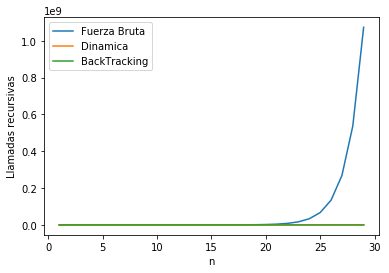
\includegraphics[width=1\textwidth]{img/llamadas/v/todosLlamadasvChico.png} % first figure itself
        \caption{Comparaci\'on de las llamadas recursivas de todos los algor\'itmos con $V = 36$}
        \label{fig:comparaTodosLlamadas}
    \end{minipage}\hfill
    \begin{minipage}{0.45\textwidth}
        \centering
        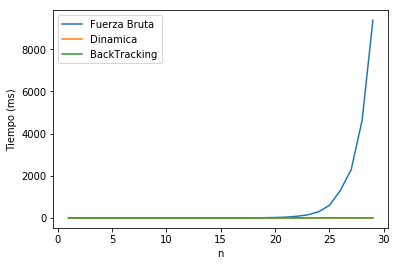
\includegraphics[width=1\textwidth]{img/tiempo/v/todosTiempo.png} % first figure itself
        \caption{Comparaci\'on de los tiempos de ejecuci\'on con $V = 36$}
        \label{fig:comparaTodosTiempo}
    \end{minipage}\hfill
\end{figure}
Tal como se puede ver en las Figuras \ref{fig:comparaTodosLlamadas} y \ref{fig:comparaTodosTiempo} resulta
inviable comparar el algor\'itmo de Fuerza Bruta con los otros dos por motivos de escala, 
raz\'on por la cual de ahora en m\'as solo voy a comparar el de Fuerza Bruta y el de Programaci\'on Din\'amica :
\begin{figure}[H] 
    \centering
    \begin{minipage}{0.45\textwidth}
        \centering 
        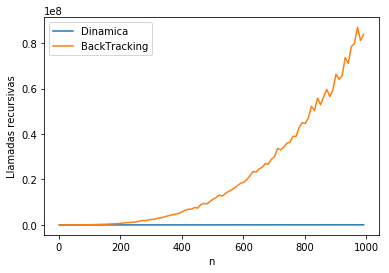
\includegraphics[width=1\textwidth]{img/llamadas/v/llamadasBackDinamicavChico.png} % first figure itself
        \caption{Comparaci\'on de las llamadas recursivas de BackTracking y Programac\'ion Din\'amica con $V = 36$}
        \label{fig:llamadasBackDinamicavChico}
    \end{minipage}\hfill
    \begin{minipage}{0.45\textwidth}
        \centering
        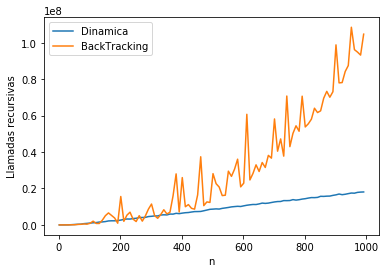
\includegraphics[width=1\textwidth]{img/llamadas/v/llamadasBackDinamicavGrande.png} % first figure itself
        \caption{Comparaci\'on de las llamadas recursivas de BackTracking y Programac\'ion Din\'amica con $V = 6048$}
        \label{fig:llamadasBackDinamicavGrande} 
    \end{minipage}
\end{figure}

\begin{figure}[H] 
    \centering
    \begin{minipage}{0.45\textwidth}
        \centering
        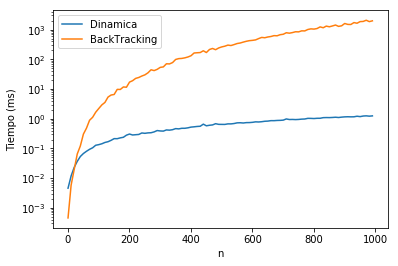
\includegraphics[width=1\textwidth]{img/tiempo/v/tiempoBackDinamicavChico.png} % first figure itself
        \caption{Comparaci\'on del tiempo de ejecuci\'on de BackTracking y Programac\'ion Din\'amica con $V = 36$}
        \label{fig:tiempoBackDinamicavChico} 
    \end{minipage}\hfill
    \begin{minipage}{0.45\textwidth}
        \centering
        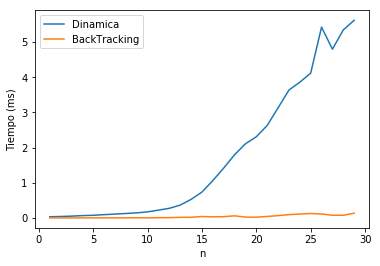
\includegraphics[width=1\textwidth]{img/tiempo/v/tiempoBackDinamicavGrande.png} % first figure itself
        \caption{Comparaci\'on del tiempo de ejecuci\'on de BackTracking y Programac\'ion Din\'amica con $V = 6048$}
        \label{fig:tiempoBackDinamicavGrande} 
    \end{minipage}
\end{figure}

Observando las Figuras \ref{fig:llamadasBackDinamicavChico}, \ref{fig:llamadasBackDinamicavGrande},
\ref{fig:tiempoBackDinamicavChico}, \ref{fig:tiempoBackDinamicavGrande} se logra
ver que los resultados obtenidos se condicen con las hip\'otesis previamente planteadas: con un valor objetivo $V$
``chico'' el algoritmo de Programaci\'on Din\'amica realiza menos llamadas (lo cual conlleva a un mayor tiempo
de ejecuci\'on) que el de BackTracking, aunque con un $V$ ``grande'' de manera que $V*n \gg 2^n$ resulta coveniente
utilizar el algoritmo de BackTracking. 
 \begin{figure}[H] 
    \centering
    \begin{minipage}{0.45\textwidth}
        \centering
        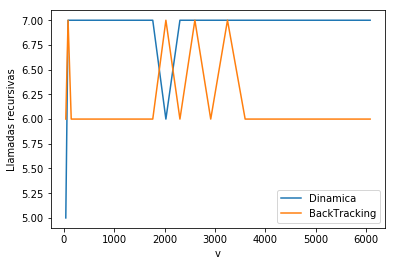
\includegraphics[width=1\textwidth]{img/llamadas/n/backDinNChico.png} % first figure itself
        \caption{Comparaci\'on entre la cantidad de llamadas recursivas entre BackTracking y Programaci\'on
        Din\'amica para $n=2$}
        \label{fig:backDinNChico} 
    \end{minipage}\hfill
    \begin{minipage}{0.45\textwidth}
        \centering 
        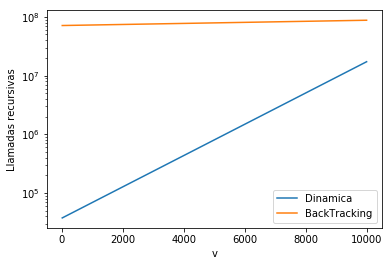
\includegraphics[width=1\textwidth]{img/llamadas/n/backDinNGrande.png} % first figure itself
        \caption{Comparaci\'on entre la cantidad de llamadas recursivas entre BackTracking y Programaci\'on
        \label{fig:backDinNGrande} 
        Din\'amica para $n=941$}
    \end{minipage}
\end{figure}

\par Por \'ultimo, analizando las Figuras \ref{fig:backDinNChico} y \ref{fig:backDinNGrande} podemos notar varias cosas que 
resultan interesantes analizar:
\par Se logra apreciar tanto la independecia de BackTracking respecto a $V$ 
(aunque esperaba que haya alguna dependencia), como la dependencia lineal de Programaci\'on din\'amica con $V$ (teniendo
en cuenta que $n$ se encuentra fijo).
\par Adem\'as, tal como se esperaba, el algor\'itmo de BackTracking se muestra superior en casos de $V$ ``grande'' y 
$n$ ``chico''.
Estimo que esto se debe a que la complejidad depende linealmente de $V$.


\subsection{Experimentaci\'on ``No Llega''}
\subsubsection{Resultados y Comparaciones}

\begin{figure}[H] 
    \centering
    \begin{minipage}{0.45\textwidth}
        \centering
        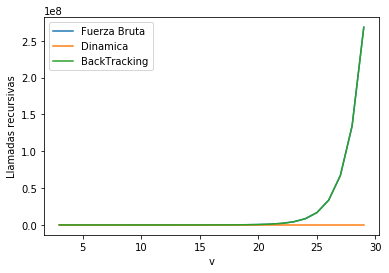
\includegraphics[width=1\textwidth]{img/nollega/todosllamadas.png} % first figure itself
        \caption{Comparaci\'on entre la cantidad de llamadas recursivas entre todos los algor\'itmos}
        \label{fig:todosllamadasnollega} 
    \end{minipage}\hfill
\end{figure}

\begin{figure}[H] 
    \centering
    \begin{minipage}{0.45\textwidth}
        \centering
        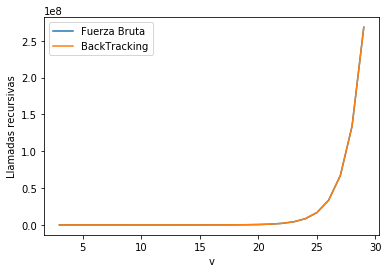
\includegraphics[width=1\textwidth]{img/nollega/backFBllamadas.png} % first figure itself
        \caption{Comparaci\'on entre la cantidad de llamadas recursivas entre los algor\'itmos de
        Fureza Bruta y BackTracking}
        \label{fig:backFBllamadasnollega} 
    \end{minipage}\hfill
    \begin{minipage}{0.45\textwidth}
        \centering
        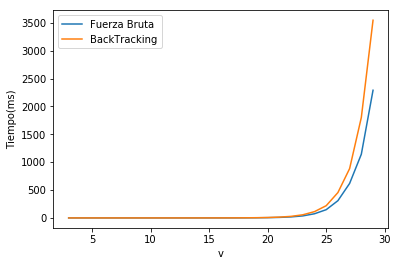
\includegraphics[width=1\textwidth]{img/nollega/backFBtiempo.png} % first figure itself
        \caption{Comparaci\'on entre el tiempo de ejecuci\'on de BackTracking y Fuerza Bruta}
        \label{fig:backFBtiemponollega} 
    \end{minipage}
\end{figure}

\par Tal como se puede ver en las Figuaras \ref{fig:todosllamadasnollega} y \ref{fig:backFBllamadasnollega}
el comportamiento de los algor\'itmos de Fuerza Bruta y BackTracking fue el esperado: realizan la misma cantidad 
de llamadas recursivas ya que en el de BackTracking no se puede realizar ninguna poda. A\'un as\', tal como
lo muestra la figura \ref{fig:backFBtiemponollega} la soluci\'on utilizando BackTracking demora considerablemente
m\'as que el otro. Estimo que esto se debe a las 4 guardas condicionales con las que cuenta (ver Pseudoc\'odigo),
raz\'on por la cual realiza $4$ operaciones extras por vez que se llama a la funci\'on. Esto resulta en $4*2^n$ 
operaciones extras en total.

\begin{figure}[H] 
    \centering
    \begin{minipage}{0.45\textwidth}
        \centering
        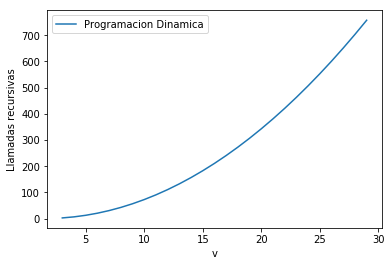
\includegraphics[width=1\textwidth]{img/nollega/dinamicallamadas.png} % first figure itself
        \caption{Cantidad de llamadas recursivas para Programaci\'on Din\'amica}
        \label{fig:dinamicallamadasnollega} 
    \end{minipage}\hfill
    \begin{minipage}{0.45\textwidth}
        \centering
        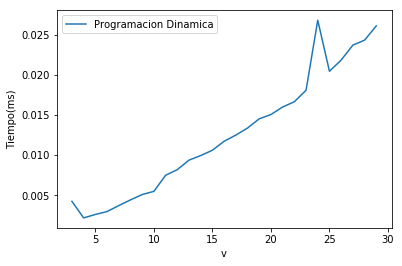
\includegraphics[width=1\textwidth]{img/nollega/dinamicatiempo.png} % first figure itself
        \caption{Tiempo de ejecuci\'on de Programaci\'on Din\'amica}
        \label{fig:dinamicatiemponollega} 
    \end{minipage}
\end{figure}

\par Por \'ultimo, para el caso de la Programaci\'on Din\'amica podemos apreciar un claro comportamiento lineal
respeco a $V$ y $n$ (recordar que $n = V-1$) en las Figuras \ref{fig:dinamicallamadasnollega} y 
\ref{fig:dinamicatiemponollega}. Adem\'as en la Figura \ref{fig:todosllamadasnollega} podemos ver que
el este algor\'itmo realiza muchas menos llamadas recursivas que el resto, validando mis hip\'otesis.